\chapter{From the Human Brain to Artificial Evolving Spiking Neural Networks} 
\label{chap:snn}

\section{Introduction}
This Chapter introduces the biophysiology of a human brain cell known as a neuron and proceeds through the historical evolution of artificial neurons and network of such neurons as computational models. Further, a brief review and the work on the evolving connectionist systems (ECOS) will be presented. This is an evolving neural network framework developed for recognising patterns from data.   

\section{The Human Brain and the Morphology of a Neuron}  
The human brain is the central processing unit of the human nervous system. It is responsible for processing, integrating, and coordinating the information it receives from the sensory organs, and making decisions as to the instructions sent to the rest of the body. The human brain is made up of a network of approximately ten billion interconnected neurons. A neuron is the basic information processing unit which receives, processes and transmits information using biochemical reactions. A typical neuron, as shown in \figurename \ref{fig:biological_neuron}, comprises three functional units, namely, dendrites, soma and axon. Dendrites are tree-like structural fibres which emanate from the cell body and provide the receptive zones for receiving the signals from other neurons. The morphology of the dendritic tree plays an important role in the integration of the synaptic inputs and influences the way the neuron processes information \citep{mel1994information}. The integration process is performed through a non-linear process of spatio-temporal summation \citep{koch1999neurobiology}. The resulting activation flows to the soma and suffers voltage attenuation, so that about half of the total charge injected into the distal dendritic site reaches the soma. The primary function of the soma is to perform the continuous maintenance required to keep the neuron functional \citep{kandel2000principles}. The part of the soma that performs the important non–linear processing of the input is known as axon hillock. If the total input produces a depolarisation up to the neural threshold, the axon hillock fires an action potential. The output signal is transmitted down the axon, which delivers it to other neurons. Some of the important characteristics of of neuron are enumerated below:

\begin{figure}
	\centering
	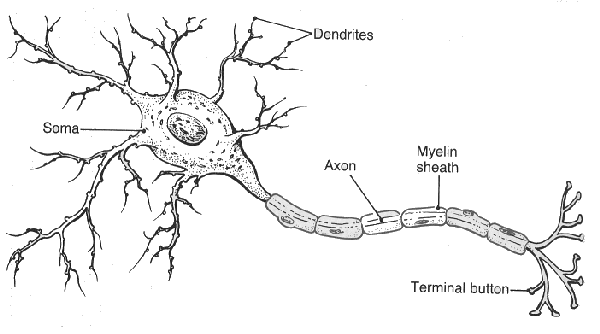
\includegraphics[width=0.7\linewidth]{fig/snn/biological_neuron.png}
	\caption{Morphology of a biological neuron (source \citet{carlson1967foundations}).}
	\label{fig:biological_neuron}
\end{figure}
\begin{itemize}
	\item Synapse: The contact point between a pre-synaptic axon and a post-synaptic dendrite or soma is known as a synapse. In a chemical synapse, arrival of action potential triggers a complex chain of biochemical reactions leading to the release of neurotransmitters. This process generates a post-synaptic potential (PSP) in the post-synaptic neuron. The internal state of a post-synaptic neuron is driven by complex integration of PSP arising from multiple such synapses. When the state of a post-synaptic neuron is sufficiently stimulated, it gives rise to an action potential or a spike which is then transmitted through the axon. Synapses are believed to be the locus of learning and memory in the brain \citep{squire1999memory}. This is where the brain is the most flexible and the most vulnerable \citep{marian2002biologically}.
	
	\item Action potential and neuron dynamics: The output generated by a biological neuron is referred to as the action potential. The action potential is an all or none electrical voltage based impulse response \citep{aur2010neuroelectrodynamics} also known as a spike. A neuronal action potential is generated when the membrane potential of the neuron reaches a threshold limit. \figurename \ref{fig:action_potential} plots a typical example of membrane potential (in mv) with time (in ms). The membrane potential starts with a resting potential of $-70 mV$. On application of a stimulus at $t=1 ms$, the membrane potential is raised above $-55 mV$ which is the threshold limit. After the stimulus is applied, the membrane potential rises to $+40$ mV. This phase is known as the depolarisation phase. The potential then drops down to $-90 mV$ at time = $3 ms$ (the repolarisation phase), and finally rises to the resting potential of $-70 mV$ is  at time = $5 ms$. The period between repolarisation and resting state is known as the refractory period during which the neuron goes into a hyperpolarisation state. During the hyperpolarised state, the neuron is incapable of firing any action potential. This mechanism stops a neuron firing spikes immediately after firing a spike.
\end{itemize}

\begin{figure}
		\centering
		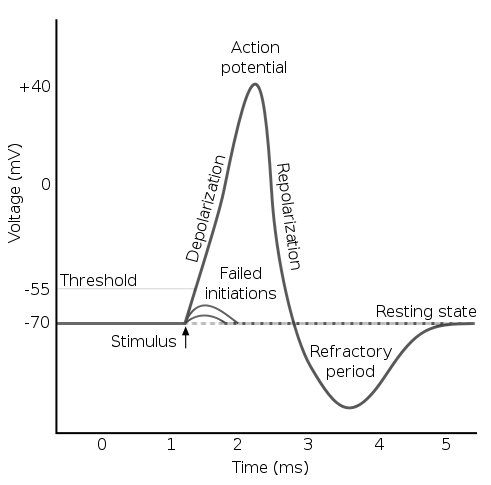
\includegraphics[width=0.6\linewidth]{fig/snn/action_potential.png}
		\caption{Dynamics of the membrane potential of a typical neuron (source \citet{Afterhyperpolarization}).}
		\label{fig:action_potential}
	\end{figure}

\subsection{Neural Encoding and Information Communication}
Neurons are thought to convey signals mainly if not exclusively through the information content of their spike-trains. A spike-train consists of a series of times at which the neuron has fired. It is possible to record spike trains from individual neurons using various electro-physiological methods in-vivo and in-vitro. Such methods have generated a good number of datasets, which, in turn, have revealed many properties of the neural computation. These properties constitute the main body of results in the rapidly growing neuroscience literature.

Neural encoding refers to the study of how neurons perceive and process information received from other neurons or through incoming stimuli. As mentioned earlier, information in a biological neuron is represented by action potentials. Even though minor variations exist in the morphology of an action potential, they are generally treated as identical stereotyped events in time. The study of neural encoding and decoding has taken massive leaps over the past decade with the availability of sophisticated invasive and non-invasive recording mechanisms from the brain cells. The curiosity regarding the nature of the neural code has been around from the beginning of neuroscience and till now, there has been no single answer towards it. Several large scale projects, such as the brain decoding project, \citep{tsien2013brain} have emerged due to progress in this area. The scientific fraternity has presented evidence over the years pointing to the existence of two major categories of neural encoding schemes: 
\begin{enumerate}
	\item Rate coding: The most classical view of the neural encoding is the rate coding and is originally shown in \citet{adrian1926impulses} through experiments conducted by hanging different weights from a muscle. They found the increase of stimulus weight increases the number of spikes recorded from the nerve. The frequency based approach of rate coding states that the firing rate of the neuron changes monotonically with the intensity or salience of the input. This also means that the randomness in the inter spike interval (ISI) in a spike train is considered as noise. This coding hypothesis can be explained by Poisson's model of random process \citep{pachitariuprobabilistic}. Out of the abundant examples of this coding scheme, the experiments conducted by \citep{hubel1959receptive, hubel1962receptive} in their ground breaking articles are the most interesting. During the experiments, light stimuli was presented to a cat and the action potentials of the primary visual cortex receptive fields were recorded over time. \figurename \ref{fig:hubel} shows how different orientation of light bars generates response of varying spike rates in the receptive fields of cat eyes. Such observations formed the basis of the rate coding scheme. 
	
	Even today, neuro-scientists often assume that useful theories can be learned about neural coding by summarising the post-stimulus time histogram (PSTH) that plots the rate of firing as a function of time. There is no doubt that rate coding seems to be the most obvious explanation of how neurons encode information. However, it is also quite evident that the firing rate as a coding scheme is highly inefficient for information processing \citep{thorpe2001spike, gautrais1998rate, van2001rate}. \citet{thorpe1989biological} argued that the primate visual cortex brain cells need to operate in less than $10\ ms$  resolution. On the other hand, the upper bound of the firing rate is $\approx 100\ Hz$, which implies that such processing can be accomplished if the individual neurons only get to fire none or one spike. The inefficiency in rate coding is caused by the requirement of precise calculation of the firing rate. \citet{gautrais1998rate} showed within a mathematical framework that during the first $10\ ms$  of computation, $n$ neurons can transmit $\log_2(n+1)$ bits of information in a rate coding scheme and $log_2(n!)$ bits of information with the alternate temporal coding scheme. The necessity of approximating firing rate from a large volume of spikes is a significant hindrance in the acceptance of this theory, especially considering the extreme efficiency of the human brain. Additionally, the refractory period of the neuron dynamics also prevents neurons from generating large numbers of spiking events within a short period.  \citet{olshausen2006other} empirically demonstrated from the electro-physiological data that rate coding V1 consumes ten times more energy to operate.  
		\begin{figure}
		\centering
		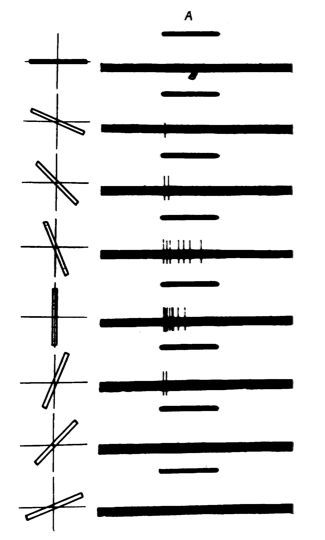
\includegraphics[width=0.3\linewidth]{fig/snn/hubel.png}
		\caption{Experimental results obtained by \citet{hubel1962receptive}. The orientation of light bars presented at various orientations are shown on the left and the spike responses are shown on the right (source \citet{hubel1959receptive}).}
		\label{fig:hubel}
	\end{figure}
	
	\item Temporal coding: Temporal encoding hypothesizes that the information is encoded in the relative timings of the spikes. This is in complete contrast to the rate coding scheme where irregularities in ISI do not arise from stochastic forces and thus are not a random process. Temporal codes employ the features of the spiking activity that cannot be described by the firing rate. For example, the time to the first spike after the stimulus onset, characteristics based on the second and higher statistical moments of the ISI probability distribution, spike randomness, or precisely timed groups of spikes (temporal patterns) are candidates of temporal coding schemes \citep{kostal2007neuronal}. Several studies have also suggested the existence of the temporal coding scheme across the animal kingdom. For fast encoding of visual stimuli in the retina cells, latency time between the stimulus onset and time to first spike is used for encoding \citep{gollisch2008rapid}. This is also known as the rank order coding \citep{van2001rate}. As with the visual system, in mitral/tufted cells in the olfactory bulb of mice, first-spike latency relative to the start of a sniffing action seem to encode much of the information about an odour. This strategy of using spike latency allows for rapid identification of and reaction to an odourant. In addition, some mitral/tufted cells have specific firing patterns for given odourants. This type of extra information could help in recognising a certain odour, but is not completely necessary, as the average spike count over the course of the animal's sniffing was also a good identifier \citep{wilson2008neural}. Along the same lines, experiments done with the olfactory system of rabbits showed distinct patterns which correlated with different subsets of odourants, and a similar result was obtained in experiments with the locust olfactory system \citep{theunissen1995temporal}.
\end{enumerate}

\section{Generations of Artificial Neuron}
It is a common understanding that primate intelligence has formed the base of artificial intelligence. The idea of mimicking or translating human intelligence into machines has been a significant ambition for the scientific community in the past centuries. The evolution of artificial neural networks has massively contributed towards realisation of that ambition. ANN is a mathematical realisation of a network of neurons or processing units that can perform complex functional mappings. Although ANNs have progressed through various stages of evolution, attempts were made only very recently to classify them into generations of neural network \citep{maass1997networks}. Due to the multiple branching of ANN research and development, this has been a challenging task. Additionally, such categorisation is subjective and dependent on what is considered as achievement. However, one such identifiable conceptual progress has been the development of mathematically-defined activation function as the information processing mechanism of an artificial neuron \citep{maass1997networks}. 

An artificial neuron has been conceived as a mathematical model of a biological neuron. \figurename \ref{fig:art_neuron} shows a block diagram of the components of an artificial neuron. Starting from the left, an ANN consists of multiple input channels. The input channels resemble the properties of dendrites in a biological neuron. These channels feed input signals (originating from pre-synaptic neurons) $\{x_1,x_2,\cdots\}$ to the processing unit of the neuron. The synaptic weights $\{w_1, w_2,\cdots\}$ define the strengths of the synapses and allows for strengthening or weakening of synapses through synaptic plasticity. The input along with the synaptic strengths are fed into the processing units which consists of the summation and activation units. These units together are responsible for mapping of the inputs $x$ to the output $y$. Next, The evolution and properties of an artificial neuron is well summarised by \citet{ghosh2009spiking}, however, for the sake of continuity, I present below, a brief overview of the three generations of computational neuron:  
\begin{figure}
	\begin{tikzpicture}[
	init/.style={
		draw,
		circle,
		inner sep=2pt,
		font=\Huge,
		join = by -latex
	},
	squa/.style={
		draw,
		inner sep=2pt,
		font=\Large,
		join = by -latex
	},
	start chain=2,node distance=13mm
	]
	\node[on chain=2] 
	(x2) {$x_2$};
	\node[on chain=2,join=by o-latex] 
	{$w_2$};
	\node[on chain=2,init] (sigma) 
	{$\displaystyle\Sigma$};
	\node[on chain=2,squa,label=above:{\parbox{2cm}{\centering Activate \\ function}}]   
	{$f$};
	\node[on chain=2,label=above:Output,join=by -latex] 
	{$y$};
	\begin{scope}[start chain=1]
	\node[on chain=1] at (0,1.5cm) 
	(x1) {$x_1$};
	\node[on chain=1,join=by o-latex] 
	(w1) {$w_1$};
	\end{scope}
	\begin{scope}[start chain=3]
	\node[on chain=3] at (0,-1.5cm) 
	(x3) {$x_3$};
	\node[on chain=3,label=below:Weights,join=by o-latex] 
	(w3) {$w_3$};
	\end{scope}
	\node[label=above:\parbox{2cm}{\centering Bias \\ $b$}] at (sigma|-w1) (b) {};
	
	\draw[-latex] (w1) -- (sigma);
	\draw[-latex] (w3) -- (sigma);
	\draw[o-latex] (b) -- (sigma);
	
	\draw[decorate,decoration={brace,mirror}] (x1.north west) -- node[left=10pt] {Inputs} (x3.south west);
	\end{tikzpicture}
	\caption{Block diagram showing components of an artificial neuron.}
	\label{fig:art_neuron}
\end{figure}
\subsection{First Generation Neurons:}
The perceptron model described by \citet{rosenblatt1958perceptron} was the beginning of the first generation of artificial neuron. The variations of this model used the perceptrons as integrate and fire units, which integrate the inputs and fired if the internal state (synaptic weighed sum of inputs) reached a threshold. Mathematically, the activation can be described by a Heavyside step function (range $\{0, 1\}$).  
\begin{equation}
f(\mathbf{x})=\left\{
\begin{array}{@{}ll@{}}
1, & \text{if}\ \mathbf{w\cdot x}+b> 0 \\
0, & \text{otherwise}
\end{array}\right.
\label{eq:perceptron_activation}
\end{equation}
\equationname \ref{eq:perceptron_activation} describes the activation of a simple perceptron. It produces binary output $y=1$ or $y=0$, if the weighed sum $\mathbf{w\cdot x}$ goes beyond $b$ or otherwise. Unlike the biological neuron, the inputs of the perceptron were real and continuous, \emph{i.e.} the magnitude of inputs contribute to the activation of the neuron. This is a primitive realisation of the rate coding scheme, \emph{i.e.} higher input causes the neuron to fire. However, the outputs were binary spikes and did not cater to the rate coding scheme. The perceptrons were also time agnostic. The inputs are always considered to be synchronous in time and it did not matter when the threshold is reached, \emph{i.e.}, as they contribute to the internal state at the same time, and hence can be directly integrated. Any events of the past do not affect the activation at the present time. 


\subsection{Second Generation Neurons:}
The second generation of neurons were developed in the 1960s as an extension of the first generation neurons. In the second generation, non linear smooth activation functions were introduced. Hence, instead of a fixed threshold value for the output determination, the outputs were proportionate within range to input signals. Tanh (\equationname \ref{eq:tanh_activation} range $(-1, 1)$) or Sigmoid (\equationname \ref{eq:sigmoid_activation} range $(0, 1)$) functions were used most often as activation functions. With this development, the outputs became real and continuous, and contrary to the first generation, the post-synaptic neurons could generate rate coded information. These neurons became extremely popular in the AI community with the introduction of feed-forward neural networks and back-propagation (BP) algorithm \citep{rumelhart1988learning}, which enabled supervised learning. Since the BP algorithm was constrained by its requirement of a continuous and differentiable activation function, a significant portion of the ensuing research became focused on finding more appropriate continuous and differentiable activation functions. This model was significantly more powerful than the one based on first generation neurons and could solve complex pattern recognition problems (the most notable early example was the XOR problem). However, the computational power of the neuron still did not reach its full potential because the temporal information about individual spikes was not represented.

\begin{equation}
f(\mathbf{x})=\frac{1}{1+e^{-(\mathbf{w\cdot x+b})}}
\label{eq:sigmoid_activation}
\end{equation}

\begin{equation}
f(\mathbf{x})=\tanh(\mathbf{w\cdot x+b})
\label{eq:tanh_activation}
\end{equation}
\subsection{Third Generation Neurons}

In the past decade, to overcome the shortcomings of the first and second generation neurons, neurons that can communicate via the precise timing of spikes or a sequence of spikes have been developed and adapted for ANNs. These neurons are known as spiking neurons. In the literature, these spiking neurons have been referred to as third generation neurons \citep{maass2001pulsed}. Similar to the first generation neurons, spiking neurons act as integrate-and-fire units and have an all or none response. The spiking neuron, however, has an inherent dynamic nature characterised by an internal state which changes with time. Each post-synaptic neuron fires an action potential or spike at the time instance that its internal state exceeds the neuron threshold. Similar to biological neurons, the magnitude of the spikes (input or output) contains no information. Rather, all information is encoded in the timing of the spikes. 

\section{Spiking Neuron Models}

The first and second generation neurons discussed in the previous Section use rather simplistic activation of the artificial neurons. The biophysical neuron models, however, are developed to quantitatively characterise neuronal behaviour based on neuron membrane potential and ion channel conductance models \citep{ghosh2009spiking}. \citet{marian2002biologically} distinguished between the two spiking neuron models by the extent of detail included in the neuron model.

\begin{enumerate}

\item Detailed neuron models: In this approach, researchers aimed at creating detailed and complex models of the neurons. \citet{de1994active, segev1998compartmental} described the chemical process at the sub-cellular level. This included ion channel and dendritic tree biophysics, synaptic interplay between excitation and inhibition, and voltage dependent events in the active dendrites \citep{mainen1998modeling}. Among all the detailed neuron models, the most prominent is the conductance based Hodgkin-Huxley model \citep{hodgkin1952quantitative}. The Hodgkin-Huxley model describes the generation of action potentials at the level of ion channels and ion current flow. It is the starting point for detailed biophysical neuron models which in general include more than the three types of currents considered by Hodgkin and Huxley. Electro-physiologists have described an overwhelming richness of different ion channels. The set of ion channels is different from one neuron to the next. The precise channel configuration in each individual neuron determines a good deal of its overall electrical properties. The model provides a detailed description of the biophysics of ionic mechanisms underlying the initiation and propagation of the neural spike. By doing this, it offers an accurate quantitative model of the physiological data. But, complex frameworks, such as this, which account for numerous ions-channels and different types of synapses are difficult to construct and analyse. An important conceptual drawback of this family of models is that their numerical complexity (e.g., solve a large number of non-linear differential equations) can prevent one from understanding which features are responsible for a particular phenomenon and which are irrelevant \citep{koch1999neurobiology}.

The Hodgkin-Huxley like models are useful in modelling point neurons. For the purpose of building detailed neuron models that can take into consideration extreme cell complexities, such as branched cable structure, the standard way is to divide a neuron into a fixed number of compartments where each compartment acts like a resistance-capacitance (RC) circuit. The RC circuits are modelled by a system of differential equations. Numerous biological neuron simulators, such as Genesis \citep{wilson1989genesis} and Neuron \citep{hines2006neuron}, implemented the compartmental models. Nonetheless, there is always a trade-off between computational cost and biological realism.

\item Formal spiking neuron models: The second direction focuses on the spiking nature of the neurons and retaining the essential elements of the behaviour being modelled, while trying to simplify the complexity of the resulting description. The main motivation for the creation of simplified models is that they allow studying more easily the computational and functional principles of neural systems.

The reduction of the detailed neuron models to formal models requires simplifications in at least two respects. First, the non–linear dynamics of spike generation must be reduced to a single ordinary differential equation and second, the spatial structure of the neuron (\emph{i.e.}, the dendritic tree) is neglected and reduced to an input \citep{gerstner2002spiking}. To support the validity of the former simplification, \citet{kistler1997reduction} demonstrated that spike generation in the Hodgkin-Huxley model can be reproduced to a high degree of accuracy (up to $90\%$) by a single variable model. Several simplified neural models have been proposed in the last decades. The leaky-integrate-and-fire (LIF) neuron is probably the best-known example of a formal neural model. It simulates the dynamics of the neuron membrane potential in response to a synaptic current by implementing an equivalent electrical circuit. The function of the integrate-and-fire circuit is to accumulate the input currents, and, when the membrane potential reaches the threshold value, to generate a spike. Immediately after emitting a pulse, the potential is reset and maintained there for an absolute refractory period.

The simplified mathematical models for spiking neurons cannot account for the entire range of computational functions of the biological neuron. Rather, they try to abstract a number of essential computational aspects of the real cell function. The essential features implemented can differ between models, as a function of what the modeller considers to be relevant and crucial for its domain study. Thus, the integrate-and-fire model focuses upon the temporal summation function of the neuron \citep{bugmann1997role}. The spike response model proposed by \citet{gerstner1998spiking} simplifies the action potential generation to a threshold process. The resonate-and-fire model \citep{izhikevich2001resonate} focuses upon the operation of the neuron in a resonating regime. By contrast with the detailed neural models, the computational strength of the spiking neurons arises from the way they interact with each other, when they work cooperatively in large networks.
\end{enumerate}

Next, I will outline some of the most prominent spiking neural network models present in the literature:

\subsection{Integrate and Fire}

The description of the Integrate and Fire (IF) and Leaky Integrate and Fire (LIF) model is adapted from \citep{gerstner2014neuronal} which serves as a comprehensive review on this topic. An IF model is described by a single variable known as membrane potential. The effect of an incoming spike on a post-synaptic neuron can be recorded using intra-cellular electrodes which measure the potential difference $v(t)$ at time $t$ between the inner and outer wall of a cell membrane. This is known as the membrane potential. In absence of any input, the neuron is said to be at rest with a constant resting membrane potential $v_{rest}$. The arrival of a spike changes the membrane potential and finally decays back to $v_{rest}$. For excitatory synapses the change is positive and for inhibitory, it is negative. The neuronal dynamics of an IF neuron can be conceived as an integration process combined with a mechanism that triggers action potential above a threshold voltage $V_{thr}$. From hereon, post-synaptic and pre-synaptic neurons will be indexed by symbols $i$ and $j$ respectively. A simple IF model can be described using: (i) A linear differential equation to describe the evolution of the membrane potential $v_i(t)$. (ii) A threshold for spike firing. 

\begin{figure}
	\centering
	\subfloat{\label{fig:if_circuit}
		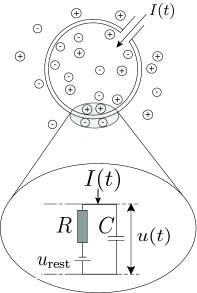
\includegraphics[width=0.45\textwidth, height=3in]{fig/snn/if_circuit.png}}
	\subfloat{\label{fig:if_response}
		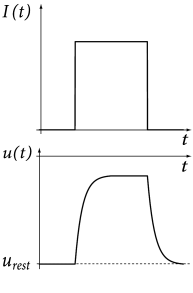
\includegraphics[width=0.45\textwidth, height=3in]{fig/snn/if_response.png}}\\
	
	\caption{Electrical properties of the passive membrane of an IF neuron. (A) A cell membrane enclosed neuron receives a positive input current $I(t)$ resulting in increase of electrical charge inside the cell. The cell membrane acts as a capacitor in parallel with a resistor which is in line with a battery of potential $v_{rest}$. (B) The reaction of the cell membrane to a step current (top) with a smooth voltage trace (source \citet{gerstner2014neuronal}).}
	\label{fig:if_neuron}
\end{figure}

\citet{gerstner2014neuronal} modelled an IF neuron as a single RC circuit (see \figurename \ref{fig:if_neuron}) following the laws of electricity. The cell membrane (insulation to the cell body) acts as a capacity of a capacitor C. Also, because the insulation is imperfect, the charge over time, slowly leaks through the cell membrane. The cell membrane hence can be characterised by a finite leak resistance R. Due to the leaky nature of the resistance, the model is also known as leaky integrate-and-fire (LIF) model.

\begin{equation}
	I(t)=I_R+I_C
	\label{eq:if_1}
\end{equation}

\begin{equation}
	I(t)=\frac{v(t)-v_{rest}}{R}+C \frac{dv}{dt}
	\label{eq:if_2}
\end{equation}

\begin{equation}
\tau_m\frac{dv}{dt}=RI(t)-[v(t)-v_{rest}]
\label{eq:if_3}
\end{equation}

\begin{equation}
v(t)=v_{rest}+RI_0[1-\exp(-\frac{t}{\tau_m})]
\label{eq:if_4}
\end{equation}


The circuit shown in \figurename \ref{fig:if_neuron} can be analysed from the law of current conservation as per \equationname \ref{eq:if_1}. This can be further rewritten as \equationname \ref{eq:if_2} by calculating $\displaystyle I_R=v_R/R$ as per Ohm's law, where $v_R=v-v_{rest}$. The $I_C$ charges capacitor C. The capacitive current can be written as $I_C=dq/dt=Cdv/dt$. Eq. \equationname \ref{eq:if_3} is the linear differential equation describing a LIF neuron's passive membrane. The trajectory of membrane potential (\equationname \ref{eq:if_4}) for a constant input current $I(t)=I_0$ starting and ending at $t=0$ and $t=\Delta$ can be derived by solving the differential \equationname \ref{eq:if_3}. The LIF neuron emits a spike denoted as $t_i^{(f)}$ generates a spike when the membrane potential $v(t)$ reaches threshold $v_{thr}$, \emph{i.e.},
\begin{equation}
	t^{(f)}: v(t^{(f)})=v_{thr}
\end{equation}

\subsection{Hodgkin-Huxley}
One of the earliest proposed (1952) models for spiking neuron is the Hodgkin-Huxley (HH) model. This model describes the influence of ion channel conductance on the spike responses of axon and was empirically studied on the axons of a Giant Squid. The choice of squid was due to its non-microscopic size. This large size was necessary as electrodes had to be inserted into the axon, in order to record the changes in electrical state experienced when neurons are active.

The HH model is described by a RC circuit connected in a parallel scheme resembling the IF model. Following \equationname \ref{eq:if_1}, the HH model rewrites it as:

\begin{equation}
C\frac{dv}{dt}=I(t)-I_R
\end{equation} 

HH model describes the resistive current as the sum of three different ion currents due to the presence of movement of sodium, potassium and leakage. The resistive current is described by \equationname \ref{eq:hh_1}.

\begin{equation}
I_R=G_{Na}m^3h(u-V_{Na})+G_K n^4(u-V_K)+G_{Leak}(u-V_{Leak})
\label{eq:hh_1}
\end{equation}

Where $V_{Na}, V_K$ and $V_{Leak}$ are known as reversible potential constants. $G_{Na}$ and $G_{k}$ are the maximum conductance of the sodium and potassium channels, while the voltage independent leak channel is represented by $G_{Leak}$. The variables $m, n$ and $h$ are gating variables described by \equationnames \ref{eq:hh_m}, \ref{eq:hh_n} and \ref{eq:hh_h}.

\begin{equation}
\frac{m}{dt}=\alpha_m(u)(1-m)-\beta_m(u)m
\label{eq:hh_m}
\end{equation}
\begin{equation}
\frac{n}{dt}=\alpha_n(u)(1-n)-\beta_n(u)n
\label{eq:hh_n}
\end{equation}

\begin{equation}
\frac{h}{dt}=\alpha_h(u)(1-h)-\beta_h(u)h
\label{eq:hh_h}
\end{equation}

where $m$ and $h$ control the sodium channel and $n$ controls the potassium channels. The function $\alpha_x(.)$ and $\beta_x(.)$ represent empirically determined voltage dynamics across capacitor $v$, are adjusted to simulate different neuron types. 

\subsection{Izhikevich}

The Izhikevich model claims to combine biological plausibility of the HH model with the lower computational complexity of the IF and LIF models \citep{izhikevich2004model}. Based on the theory of dynamic systems, the dynamics of this model are governed by two equations:

\begin{equation}
	\frac{dv}{dt}=0.04v^2+5v+140-u+I
\end{equation}
where $u$ is a membrane recovery variable providing negative feedback for $v$; variables $u$ and $v$, and parameters $a, b, c$ and $d$ are dimensionless. The input stimuli in the form of input current is represented by $I$. When the membrane potential reaches the (fixed) threshold $v_{thr}=30 mV$, the neuron spikes and resets $u$ and $v$ as:

\begin{equation}
if v\geq 30 mV\left\{
\begin{array}{@{}ll@{}}
v\leftarrow c, & \\
u\leftarrow u+d, & 
\end{array}\right.
\end{equation}

Dependent on parameters $a$ (decay rate of membrane potential), $b$ (sensitivity of membrane recovery), $c$ and $d$ (reset values of $v$ and $u$ respectively), a huge variety of neuronal types can be modelled with relative ease. 

It can be observed that the mathematical representation of the biological neurons are extremely complex and focus on mimicking the biological properties accurately. This direction of work focuses on discoveries of biophysical properties of neurons and the human brain through simulations. The work of this thesis is, however, not intended to follow that direction. This work focuses on using the spiking properties of the biological neurons, interwoven together in a network for solving pattern recognition problems. Therefore, it is necessary to compare the capabilities of the spiking neuron models in regards to the biological plausibility and complexity vs computational cost. \citet{izhikevich2004model} presented an insightful comparison of over twenty spiking neuron models in this regard. Izhikevich, in this article, compared the presence or absence of $22$ categories of biological properties, such as tonic spiking, phasic spiking, spike latency and chaos in the spiking neuron models. \figurename \ref{fig:izhikevich} shows the comparison of spiking neuron models presented in \citep{izhikevich2004model}. The biological plausibility on the Y axis is measured by the total number of biological properties (out of 22 different categories) present in the neuron model. The X axis plots the implementation cost of the neuron model by the number of floating point operations (FLOPS). It can be observed that out of many models proposed in the literature, Hodgkin-Huxley and integrate-and-fire neurons, reside at the extremity of the evaluation landscape. The choice of neuron models, as argued in \citep{izhikevich2004model} really depends on the goal. If the goal is to simulate a large number of neurons interacting within a network, efficiency plays an important role. Variations of IF models are suitable for this purpose. For the rest of this thesis, variations of the IF model are used and discussed.  
\begin{figure}
	\centering
	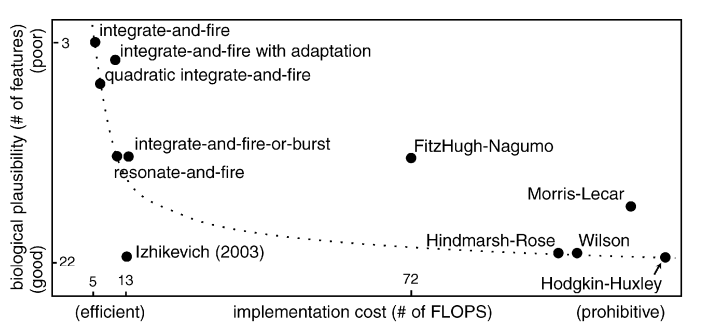
\includegraphics[scale=0.8]{fig/snn/izhikevich.PNG}
	\caption{Comparison of spiking neuron models in the evaluation landscape of biological plausibility and implementation cost (source \citet{izhikevich2004model}).}
	\label{fig:izhikevich}
\end{figure}


\section{Spiking Neural Networks}

The phenomenological models of spiking neurons described earlier can be simplified to lesser realistic models where spikes are not modelled which leads to the first two generations of the neurons. Of course, the computational load reduces drastically along with biological plausibility. For decades, the modelling of the neurons was limited by the available computing power because the hardware was unable to support large ANNs based on detailed neuronal models. This limitation dictated the design of the learning algorithms. Subsequently, even when advances were made in computing power, proportionate advances were not made in the complexity of the neuronal models because the existing learning algorithms were not compatible with the detailed models. 

Accordingly, two distinct research areas emerged. The field of Artificial Neural Networks concentrated on the behaviour of large networks of neuron-like processing units (\emph{i.e.}, the second generation neurons), which were primitive and oversimplified formulations of biological neurons. However, it was demonstrated that even such networks were capable of learning using pseudo-realistic learning algorithms, such as backpropagation. ANNs were applied with great success to pattern recognition, classification, and pattern completion tasks in a wide variety of areas. The other field became known as Computational Neuroscience. Within this broad interdisciplinary field, the detailed biophysical and phenomenological models were primarily used in relatively smaller networks to study electro-physiological processes, pattern generation, and the dynamic behaviour of small groups of neurons. There have also been studies involving very large numbers of interconnected biophysical neuron models. However, it has not been possible to use such networks of detailed neurons in a manner similar to ANNs for large real-world pattern recognition and classification tasks. 

Modern advances and the accessibility of computing resources have increased the overlap between the two fields. On one hand, the processing units, networks, and learning algorithms for ANNs have
become biologically more realistic. On the other hand, networks of biophysical neurons have become increasingly larger in size and the biophysical models, more detailed. The available computing power still limits the use of the detailed models in large biophysical neural networks for pattern recognition and classification tasks. As the computing power becomes more readily available, suitable learning algorithms are also being developed for such models. The development of Spiking Neural Networks (SNN) was the next logical step towards achieving this goal.

Simply stated, SNNs are networks of spiking neurons. The SNN is architecturally similar to that of a traditional ANN. The processing units, however, are spiking neurons, typically modelled by a phenomenological model, such as a Spike Response Model. As discussed earlier, the use of the biophysical models in certain applications of SNNs is less common due to the computational burden.

\section{Neuromorphic Computing Beyond von Neumann Hardware Architecture}

This Section is an adaptation of the article \citep{kasabov2016neumann} published  in 2016. The tremendous push of AI towards emulation of real intelligence has been sustained by the realisation of Moore's law \citep{schaller1997moore}, which states that the processing power of central processing units (CPU) will double every couple of years. The scalable computer architecture proposed by John von Neumann in 1945 as part of the draft of EDVAC computer \citep{randell2013origins} had to play a substantial role in accomplishing the continuous miniaturisation of the CPU chips. In more recent years, CPU chip manufacturing companies have spent billions of dollars in CMOS technology to shrink the transistor size to a minuscule ($\approx 14$ nanometres) and thus keep Moore's law alive. It is evident that this is non-sustainable and as per well-supported predictions will reach its boundary in the next three to five years \citep{toumey2016less}. The literature suggests that the ongoing effort to enhance the traditional von Neumann architectures are unlikely to lower simulation runtimes significantly, as single and multi-core architectures are reaching a state of saturation in terms of transistor size \citep{thompson2006moore}, energy consumption \citep{esmaeilzadeh2011dark} and communication \citep{perrin2011complexity}. 

The Von Neumann architecture is a multi-modular design based on rigid physically separate functional units. It specifically consists of three different entities:
\begin{itemize}
	\item Processing unit: The processing unit can be broken down into several sub-units, the arithmetic and logical unit (ALU), the processing control unit and the program counter. The ALU computes the arithmetic logic needed to run programs. The control unit is used to control the flow of data through the processor. 
	\item I/O unit: The i/o unit essentially encompasses all I/O the computer could possibly do (printing to a monitor, to paper, inputs from a mouse or keyboard, and others.).
	\item Storage unit: The storage unit stores anything the computer would need to store and retrieve. This includes both volatile and non volatile memory.
\end{itemize}

These units are connected over different buses like data bus, address bus and control bus. The bus allows for the communication between the various logical units. Though very robust, this architecture inherently suffers from the bottleneck created due to the constant shuffling of the data between the memory unit and the central processing unit. This bottleneck leads to rigidity in the architecture as the data needs to pass through the bottleneck in a sequential order. An alternate solution of parallelising the computers has been proposed where millions of processors are interconnected. Despite the increase in processing power, this solution is still limited by the bottleneck in its core elements \citep{schuller2016vonneumann}.

\begin{table}
	\centering
	\caption{A comparison of the key contrasts between von Neumann and neuromorphic computing paradigm.}
	\label{tab:comp}
	\resizebox{\textwidth}{!}{
	\begin{tabular}{@{}|l|ll|@{}}
		\toprule\toprule
		Properties & \textbf{von Neumann} & \textbf{Neuromorphic} \\ \midrule
		Representation of the data & Sequence of binary numbers & Spike (event) timings \\ 
		Memory & \begin{tabular}[c]{@{}l@{}}Volatile and non-volatile\end{tabular} & \begin{tabular}[c]{@{}l@{}}Long and short term memory\end{tabular} \\
		Plasticity (Learning) & No & \begin{tabular}[c]{@{}l@{}}Long, short term potentiation and depression\end{tabular} \\
		Processing & \begin{tabular}[c]{@{}l@{}} Deterministic, centralised and sequential\end{tabular} & \begin{tabular}[c]{@{}l@{}} Stochastic, decentralised and parallel\end{tabular} \\ \bottomrule \bottomrule
	\end{tabular}}
\end{table}

The saturation in the scalability of the von Neumann architecture led to developments in computer and computing architectures. Neuromorphic computing was coined by Carver Mead \citep{mead1990neuromorphic} in the 1980s and further developed in a new paradigm of computing. As the name `neuromorphic' suggests, this is inspired by the human brain. Moreover, as the existence of AI is complimented by computing architectures, having a real neuromorphic computer architecture oriented processing unit is a step towards the development of highly neuromorphic AI. The focus of neuromorphic hardware systems are to model the behaviour of the biological neurons in digital or analog circuits. It also draws great inspiration from our brain's ability to manage tens of billions of processing units connected by the hundreds of trillions of synapses using tens of watts of power on average. The large network of the processing units (neurons) in the brain are in a true sense a mesh. The data is transmitted over the network via the mesh of synapses seamlessly. Architecturally, the presence of the memory and the processing unit as a single abstraction is uniquely advantageous leading to dynamic, self-programmable behaviour in complex environments \citep{schuller2016vonneumann}. The highly stochastic nature of computation in our brain is a very significant divergence from the bit-precise processing of the traditional CPU. The neuromorphic computing hence aspires to move away from the bit-precise computing paradigm towards the probabilistic models of simple, reliable, power and data efficient computing \citep{calimera2013human} by implementing neuromorphic principles, such as spiking, plasticity, dynamic learning and adaptability. This architecture morphs the biological neurons, where the memory and the processing units are present as part of the cell body leading to the decentralised presence of memory and processing power over the network. There is a significant interest in such hardware implementations of SNN due to many factors. The primary factor being the massive power efficiency -somewhere in the order of 20 watts- for its ability to learn and operate in a stochastic environment. Such systems can be broadly categorised in one of the families of Application-Specific Integrated Circuit (ASIC), Field Programmable Gate Array (FPGA), or digital systems. \tablename \ref{tab:comp} lists some fundamental characteristics of the von Neumann and neuromorphic architecture.

\begin{table}
	\centering
	\caption{Comparison of the key features of the popular neuromorphic systems and human brain. The details are adapted from \citep{scott2015thesis, furber2016large}.}
	\label{tab:neuromorhic_hardware_comparsion}
	\resizebox{\textwidth}{!}{%
		\begin{tabular}{@{}l|llll@{}}
			\toprule
			\toprule
			Feature & Human brain & SpiNNaker \citep{furber2014spinnaker} & Zheijang FPGA \citep{li2005multi} & TrueNorth \citep{hsu2014ibm} \\ \midrule
			Type & Biological & Programmable digital & FPGA & Fixed Digital \\ 
			Neuron model & Diverse & Programmable & LIF & LIF \\ 
			Synapse model & Diverse & Programmable & Programmable & Binary \\ 
			Max \# neurons & $100B$ & $16K$ & $2048$ & $1M$ \\ 
			Max \# synapses & $10^{15}$ & $14M$ & $4.2M$ & $256M$ \\ 
			Runtime plasticity & yes & Programmable & No & No \\ 
			Energy per connection & $10$fJ & $10$nJ & Unknown & $25$pJ \\ 
			Biological speed up & $1x$ & $1x$ & $1x$ & $1x$ \\ 
			\bottomrule
			\bottomrule
		\end{tabular}%
	}
\end{table}

A number of large-scale neuromorphic systems have emerged over recent years taking advantage of the enormous transistor resources now available on a single microchip. The enhanced capabilities of the neuromorphic systems enable modellers to contemplate building models of complete brains of animals from insects up to smaller mammals, or substantial sub-areas of the human brain, and the same systems also offer platforms capable of supporting new scales of cognitive architecture \citep{furber2016large}. A tabular comparison of the neuromorphic hardware platforms are adapted from \citep{scott2015thesis} and shown in \tablename \ref{tab:neuromorhic_hardware_comparsion}.

\textbf{SpiNNaker}: The SpiNNaker hardware, developed as part of the Human Brain Project is a massively parallel digital computer whose communication infrastructure is motivated by the the objective of modelling massively scalable SNN with the  brain like connectivity profile in biological real time. In many respects, SpiNNaker resembles conventional supercomputers, with the following differences:
\begin{itemize}
	\item The processors in SpiNNaker are mobile IC chips.
	\item The communication protocol in SpiNNaker is brain inspired and is optimised for broadcasting large quantities of small data packets to destinations in a stochastic manner.
\end{itemize}
The SpiNNaker system is designed around a plastic ball grid array package which incorporates a custom processing chip and a $128$ Mbyte SDRAM memory chip. The processing chip contains $18$ ARM968 processing cores, each with $23$ Kbytes of instruction memory and $64$ Kbytes of data memory, a multicast packet router and sundry support components \citep{furber2016large}. The SpiNNaker communication fabric is based on a 2D triangular mesh with each node formed from a processor layer and a memory layer. The routing is based upon packet-switched Address Event Representation and relies on the fact that the connections from a particular neuron are static, or at most slowly
changing. Each neuron can route through a unique tree, though in practice routing is based on populations of neurons rather than individual neurons, and the restricted size of each routing table makes this optimisation necessary in most cases. In addition to the hardware system, the project also developed numerous high level neural description language, such as PyNN \citep{davison2008pynn} and Nengo \citep{bekolay2013nengo} for application development on SpiNNaker.

\textbf{IBM TrueNorth}: The IBM TrueNorth chip is the hardware developed under the DARPA SYNAPSE programme aimed at developing dense, power-efficient hardware for cognitive applications. This hardware consists of a $5.4$ million transistor $28$ nm CMOS chip with $4096$ cores, where each core is made up of $256$ neurons each having $256$ synaptic inputs \citep{cassidy2013cognitive}.

The design of the TrueNorth core is a $256 \times 256$ cross-bar which selectively connects incoming
neural spike events to outgoing neurons. The cross-bar inputs are coupled via buffers that can insert axonal delays. The outputs from the cross-bar couple into the digital neuron model, which implements a form of IF algorithm with $23$ configurable parameters that can be adjusted to yield a range of different behaviours, and digital pseudo-random sources are used to generate stochastic behaviours through modulating the synaptic connections, the neuron threshold and the neuron leakage. Neuron spike event outputs from each core follow individually-configurable point-to-point routes to the input to another core, which can be on the same or another TrueNorth chip. Where a neuron output is required to connect to two or more neurosynaptic cores, the neuron is simply replicated within the same core. The TrueNorth hardware is supported by a software emulator, which, exploiting the deterministic nature of the hardware, can be relied upon to predict the performance of the hardware exactly.

Apart from these two systems that rose to prominence, numerous other neuromorphic hardware systems are being constantly developed. Some of the systems worth a mention include Neurogrid (Stanford University) \citep{boahen2006neurogrid,}, BrainScaleS (University of Heidelberg) \citep{markram2011introducing}, and multi-PWM pulse generator (Zheijiang University) \citep{li2005multi}.

\section{Brief Review of SNN Software Implementations}
The number of software implementations that have appeared, as a result of ongoing research in the area of ANN and SNN, is ever growing. These software packages are developed for two main purposes:

\begin{itemize}
	\item Data analysis: They are aimed at analysing real-world data derived from practical applications. These software use a relatively simple static architecture, hence are easily configurable and easy to use. A few examples of such software are: multi-layer perceptron (MLP) \citep{baum1988capabilities}, RBF network \citep{park1991universal}, Probabilistic network (PNN) \citep{specht1990probabilistic}, Self organising maps (SOM) \citep{kohonen1998self}, Evolving connectionist systems, such as DENFIS and EFuNN \citep{kasabov2007evolving}. These software are either available as independent open source APIs, such as NeuCom \citep{neucom}, PyBrain (python) \citep{schaul2010pybrain}, Fast Artificial Neural Network (C++) \citep{nissen2000fast}, or as part of a data analytics suite like Weka \citep{hall2009weka}, Knime \citep{berthold2008knime}, Orange \citep{demvsar2004orange} and so on.
	\item Research and development systems: As opposed to data analysis software, they are complex in behaviour, and require expert knowledge for usage and configuration. The majority of the existing SNN software belong to this class of ANN.
\end{itemize}

NEURON \citep{hines1997neuron}: Neuron is aimed at simulating a network of detailed neurological models. Its ability to simulate biophysical properties, such as multiple channel types, channel distributions, ionic accumulation and so on, renders it well suited for biological modelling \citep{brette2007simulation}. It also supports parallel simulation environment through: (1) distributing multiple simulations over multiple processors, and (2) distributing models of individual cells over multiple processors.

PyNEST \citep{eppler2008pynest}: The neural simulation tool (NEST) is primarily developed in C++ to simulate a heterogeneous network of spiking neurons. NEST is implemented to ideally model neurons in the order of $10^4$ and synapses in the order of $10^7$ to $10^9$ on a range of devices from single core architectures to supercomputers. NEST interfaces with python via implementation of PyNEST. PyNEST allows for greater flexibility in simulation setup, stimuli generation and simulation result analysis. A `node' and a `connection' comprise the core elements of the heterogeneous architecture. The flexibility to simulate `a neuron', `a device' or `a subnetwork (which can be arranged hierarchically)' as a node, provides a major improvement over \citep{pecevski2009pcsim}. Due to the bottom-up approach of network simulation, the software allows for individually configurable neuron states and connection setup. 

Circuit Simulator \citep{natschlager2003computer}: The circuit simulator is a software developed in C++ for simulation of heterogeneous networks with major emphasis on high-level network modelling and analysis, as opposed to \citep{hines1997neuron}. The C++ core of the software is integrated with Matlab based GUI, for ease of use and analysis. CSIM enables the user to operate both spiking and analog neuron models along with mechanisms of spike and analog signal transmission through its synapse. It also performs dynamic synaptic behaviour by using short and long-term plasticity. In 2009, circuit simulator was further extended to parallel circuit simulator (PCSIM) software with the major extension being implementation on a distributed simulation engine in C++, interfacing with Python based GUI.

Neocortical Simulator \citep{drewes2005brainlab}: NCS or Neocortical Simulator is a SNN simulation software developed for simulating mammalian neocortex \citep{brette2007simulation}. During its initial development, NCS was a serial implementation in Matlab but later rewritten in C++ to integrate distributed modelling capability \citep{wilson2001parallel}. As reported in \citep{brette2007simulation}, NCS could simulate in the order of 106 single compartment neurons and $1012$ synapses using STP, LTP and STDP dynamics. Due to the considerable setup overhead of the ASCII-based files used for the I/O, a Python-based GUI scripting tool called BRAINLAB \citep{drewes2005brainlab} was later developed to process I/O specifications for large scale modelling.

Oger Toolbox \citep{pecevskioger}: Oger toolbox is a Python-based toolbox, which implements modular learning architecture on large datasets. Apart from traditional machine learning methods such as PCA and ICA, it also implements SNN based reservoir computing paradigm for learning from sequential data. This software uses a single neuron as its building block, similar to the implementation in \citep{eppler2008pynest}. A major highlight of this software includes the ability to customise the network with several non-linear functions and weight topologies, and a GPU optimised reservoir using CUDA.

BRIAN \citep{goodman2009brian,goodman2010code}: Brian is a SNN simulator application programming interface written in Python. The purpose of developing this API is to provide users with the ability to write quick and easy simulation code \citep{goodman2010code}, including custom neuron models and architecture. The model definition equations are separated from the implementation for better readability and reproducibility. \citet{goodman2009brian} also emphasise the use of this software in teaching a neuroinformatics course \citep{diesmann1999stable}. A major limitation of BRIAN is, however, the requirement of Python knowledge to run the simulation, and the lack of GUI for the non-technical user community. 



\section{Evolving Connectionist System}
It is beyond any speculation that AI and neuromorphic hardware systems belong to a unified symbiotic ecosystem, where a neuromorphic hardware is truly neuromorphic if and only if it has dynamic learning, adaptation and creativity incorporated in the framework. On the other hand neuromorphic learning systems are paradigm shifting in machine learning where it is not only about accurate performance, but also about performing it economically using limited resources.

Subsequently, I will concentrate on the principle and evolution of the Evolving Connectionist System (ECOS) with emphasis on our work in evolving spiking neural network (eSNN). The rest of the Chapter is an adaptation of our work presented in \citep{arya2016cyber} along with an article under review. 

\subsection{Principles of ECOS}
The human brain's unique ability to combine low level learning within an interconnected framework and high level rule abstraction leads to the learning of abstract concepts. ECOS is inspired by this very concept and aims at training neural networks for deriving abstract knowledge representations that explains data and can be used as an interpretable knowledge-based system. The ECOS was developed as a trend in neural networks and computational intelligence by \citet{kasabov2001evolving} and incorporated in many novel computational methods over the last few decade across different application domains. Some classical example of ECOS systems are EFuNN \citep{kasabov1998evolving} and DENFIS \citep{kasabov2002denfis}, where classical McCulloch and Pitts neuron models are used to perform pattern recognition in single dimensional scalar data. ECOS principle was propagated further to evolving spiking neural networks (eSNN) that used spiking neuron models and temporal spike sequences as data representation. The eSNN was architected primarily as a visual pattern recognition system. The first eSNNs were based on the Thorpe’s `time to first spike' rule \citep{thorpe2001spike}, in which the importance of early spikes (after the onset of a certain stimulus) is boosted, called rank-order encoding and learning. \cite{kasabov2013dynamic} further proposed dynamic eSNN (deSNN), which combines rank order encoding of eSNN with dynamic Hebbian spike-time based learning. The main advantage of the eSNN when compared with other supervised or unsupervised SNN models is that it is computationally inexpensive due to the one-pass nature of the learning algorithm and boosts the importance of the order in which input spikes arrive, thus making the eSNN based algorithms suitable for on-line learning with a range of applications. For a comprehensive study of ECOS and eSNN see \citep{watts2009decade, wysoski2010evolving}. I, in collaboration with The Institute of Development and Research in Banking Technology, India, have used eSNN in applications of automatic cyber fraud detection and stock price movement prediction case studies. In the following two Sections, the results that have been obtained will be summarised from these two studies. The detail of each of the studies can be found in Appendix \ref{app:eSNN_cyber} and \ref{app:eSNN_stock}
\subsection{Application of eSNN in Forecasting Stock Price Movement}      

Prediction of the stock price index and its trend are considered challenging tasks due to their complexity, non-linearity, dynamic and chaotic nature. In addition, the stock market behaviour is also influenced by socio-political movements, investor psychology, and so on. Although many researchers have explored several forecasting techniques, it is for the first instance that eSNN has been employed to develop a computational model for the stock market movement trend prediction. In this study, two computational models are proposed, namely, CUDA-SI-eSNN, which is a parallel CUDA implementation of the standard eSNN architecture. The second algorithm, known as SW-eSNN, is the incremental learning of eSNN using a sliding window of data. Appendix \ref{app:eSNN_stock} describes the motivation behind this study along with descriptions of the proposed SI-eSNN, CUDA-SI-eSNN and SW-eSNN architectures along with the formal description of the algorithms. 

\subsubsection{Dataset Description and Experiments with the SI-eSNN and the CUDA-eSNN Models}
\label{sec:dataset}

The datasets used in this study are obtained from QUANDL \citep{Quandl2017financial}, \citep{Bse2017financial}, and \citep{Nse2017financial}. These datasets cover stock market indices of different countries: BSE, Nikkie-225, NIFTY-50, S\&P-500, Dow-Jones, NYSE-Amex, DAX, NASDAQ and Shanghai stock exchange. In this study, thirteen technical indicators have been selected as input variables based on earlier research done in \citep{kim2003financial,patel2015predicting,kara2011predicting}. The direction of daily stock price index is categorised as `UP' or `DOWN'. If the stock price index at time $t$ is higher than that at time $t+1$, then the trend is `DOWN'. If the stock price index at time t is lower than that at time $t+1$, then the trend is `UP'. The number of instances of each of the stock index data is given in \tablename \ref{tab:num_instance_up_down}. The details about selected indicators is given in \tablename \ref{tab:tech_indicators} and the summary statistics of selected technical indicators for each stock indices are provided in the supplementary information.

In the experiments, the first $70\%$ of the temporal stock data represented by the $13$ indicators on a daily basis are used as input variables for training the SI-eSNN and the CUDA-SI-eSNN models and the future $30\%$ of the time series stock data is used to test the model accuracy. Experiments in the present study were carried on systems with $32$ GB RAM and eight cores. The GPU device used for all of our experiment is GeForce GT730.  The details of the GPU device is given in \tablename \ref{tab:gpu_specs}. 

Classification accuracy and AUC scores were used to evaluate the performance of both eSNN and CUDA-SI-eSNN models. Sensitivity and specificity are used to assess the AUC score. In addition to the sensitivity, specificity and accuracy equations described earlier, the AUC score can be defined as:

\begin{equation}
AUC\ score=\frac{Sensitivity+Specificity}{2}
\end{equation}



% -----------------------------------------


\begin{table}
	\centering
	\caption{Accuracy and AUC of CUDA-eSNN model with Gaussian Distribution for different stock indices.}
	\label{tab:accuracy}
	\resizebox{\textwidth}{!}{\begin{tabular}{clllllllllllllll}
			\toprule[1.25pt]
			\multicolumn{1}{c}{Datasets}     & \multicolumn{3}{c}{BSE}                        & \multicolumn{3}{c}{Nikkie-225} & \multicolumn{3}{c}{NASDAQ}   & \multicolumn{3}{c}{NIFTY-50} & \multicolumn{3}{c}{S\&P-500} \\
			
			\midrule
			No. of Gaussian Receptive Fields & Acc. ($\%$) & T.T (Sec) & AUC  & Acc. ($\%$)  & T.T (Sec)  & AUC  & Acc. ($\%$) & T.T (Sec) & AUC  & Acc. ($\%$) & T.T (Sec) & AUC  & Acc. ($\%$) & T.T (Sec) & AUC  \\
			\midrule
			$3$                                & $82.17$     & $0.84$      & $0.82$ & $81.57$      & $3.3$        & $0.81$ & $84.46$     & $0.89$      & $0.84$ & $76.85$     & $0.61$      & $0.76$ & $82.96$     & $8.51$      & $0.82$ \\
			$4$                                & $85.71$     & $1.06$      & $0.86$ & $82.53$      & $4.67$       & $0.82$ & $85.43$     & $1.1$       & $0.85$ & $79.96$     & $0.7$       & $0.79$ & $83.74$     & $9.77$      & $0.83$ \\
			$5$                                & $83.88$     & $1.25$      & $0.83$ & $80.33$      & $5.96$       & $0.8$  & $84.22$     & $1.23$      & $0.84$ & $80.13$     & $0.69$      & $0.8$  & $81.16$     & $11.59$     & $0.81$ \\
			$6$                                & $85.59$     & $1.36$      & $0.85$ & $84.41$      & $7.15$       & $0.84$ & $84.22$     & $1.24$      & $0.83$ & $77.37$     & $0.79$      & $0.77$ & $82.72$     & $13.78$     & $0.82$ \\
			$7$                                & $87.05$     & $1.39$      & $0.87$ & $80.88$      & $8.06$       & $0.80$  & $\mathbf{85.92}$     & $\mathbf{1.53}$      & $\mathbf{0.86}$ & $82.55$     & $0.81$      & $0.82$ & $82.53$     & $18.95$     & $0.82$ \\
			$8$                                & $85.47$     & $1.55$      & $0.85$ & $86.15$      & $8.91$       & $0.85$ & $81.79$     & $1.55$      & $0.81$ & $82.03$     & $0.84$      & $0.81$ & $84.03$     & $22.05$     & $0.84$ \\
			$9$  & $\mathbf{88.76}$     & $\mathbf{1.65}$      & $\mathbf{0.88}$ & $82.12$      & $9.68$       & $0.82$ & $84.7$      & $1.67$      & $0.84$ & $81.69$     & $0.93$      & $0.81$ & $82.16$     & $29.05$     & $0.82$ \\
			$10$                               & $86.08$     & $1.75$      & $0.86$ & $\mathbf{87.12}$      & $\mathbf{10.6}$       & $\mathbf{0.87}$ & $85.92$     & $1.84$      & $0.85$ & $83.93$     & $0.99$      & $0.83$ & $84.13$     & $35.7$      & $0.84$ \\
			$11$                               & $88.64$     & $1.78$      & $0.88$ & $83.73$      & $11.58$      & $0.83$ & $84.7$      & $1.91$     & $0.84$ & $80.31$     & $1.05$      & $0.8$  & $84.5$      & $39.36$     & $0.84$ \\
			$12$                               & $87.91$     & $1.88$      & $0.88$ & $86.11$      & $12.41$      & $0.86$ & $83.49$     & $2.04$      & $0.83$ & $82.38$     & $1.08$      & $0.82$ & $81.26$     & $46.94$     & $0.81$ \\
			$13$                               & $88.4$      & $2$         & $0.88$ & $83.68$      & $13.15$      & $0.83$ & $84.22$     & $2.19$      & $0.84$ & $\mathbf{84.45}$     & $\mathbf{1.18}$      & $\mathbf{0.84}$ & $\mathbf{84.74}$     & $\mathbf{51.51}$     & $\mathbf{0.84}$ \\
			$14$                               & $87.91$     & $2.25$      & $0.88$ & $86.57$      & $14.04$      & $0.86$ & $83.73$     & $2.19$      & $0.83$ & $81$        & $1.22$      & $0.8$  & $84.13$     & $51.88$     & $0.84$ \\
			\bottomrule[1.25pt]
	\end{tabular}}
	\vspace{0.5ex}
	\raggedright $\ast$Acc.=Accuracy, $\ast$T.T = Training Time
\end{table}

% -----------------------------------------

\begin{table}
	\centering
	\caption{Accuracy and AUC of CUDA-eSNN model with Gaussian Distribution for different stock indices (Continued).}
	\label{tab:accuracy_cont}
	\resizebox{\textwidth}{!}{\begin{tabular}{@{}cllllllllllll@{}}
			\toprule[1.25pt]
			\multicolumn{1}{c}{}             & \multicolumn{3}{c}{Sanghai Stock Exchange} & \multicolumn{3}{c}{Dow-Jones} & \multicolumn{3}{c}{NYSE-Amex} & \multicolumn{3}{c}{DAX-Index} \\
			\midrule
			No. of Gaussian Receptive Fields & Acc. (\%)      & T.T (Sec)      & AUC      & Acc. (\%)  & T.T (Sec) & AUC  & Acc. (\%)  & T.T (Sec) & AUC  & Acc. (\%)  & T.T (Sec) & AUC  \\ \midrule
			3                                & 77.48          & 1.68           & 0.77     & 75.31      & 0.83      & 0.74 & 78.37      & 2.01      & 0.77 & 79.23      & 2.67      & 0.79 \\
			4                                & 78.14          & 2.08           & 0.78     & 76.59      & 0.93      & 0.76 & 84.04      & 2.5       & 0.83 & 77.64      & 4         & 0.77 \\
			5                                & 80.74          & 3.13           & 0.8      & 75.31      & 0.96      & 0.74 & 82.75      & 3.67      & 0.81 & 81.55      & 5.12      & 0.81 \\
			6                                & 80.37          & 3.3            & 0.8      & 78.38      & 1.05      & 0.78 & 80.56      & 3.96      & 0.8  & 82.07      & 5.79      & 0.81 \\
			7                                & 79.92          & 3.7            & 0.79     & 79.79      & 1.23      & 0.79 & 82.62      & 4.4       & 0.82 & 78.41      & 6.43      & 0.78 \\
			8                                & 79.18          & 3.73           & 0.79     & 79.28      & 1.46      & 0.79 & 77.79      & 4.7       & 0.77 & 82.22      & 7.22      & 0.81 \\
			9                                & 79.48          & 3.76           & 0.79     & 78.51      & 1.49      & 0.78 & 82.78      & 5.1       & 0.83 & 82.53      & 7.76      & 0.82 \\
			10                               & 80.37          & 4.8            & 0.8      & 77.74      & 1.59      & 0.77 & 83.65      & 5.51      & 0.82 & 82.07      & 8.48      & 0.81 \\
			11                               & \textbf{82.66}          & \textbf{5.2}            & \textbf{0.82}     & 77.62      & 1.69      & 0.77 & 81.78      & 6.05      & 0.81 & 83.41      & 9.11      & 0.83 \\
			12                               & 79.77          & 5.33           & 0.79     & 79.28      & 1.77      & 0.79 & 86.29      & 6.45      & 0.85 & \textbf{84.9}       & \textbf{9.66}      & \textbf{0.84} \\
			13                               & 79.7           & 5.9            & 0.79     & \textbf{81.2}       & \textbf{1.84}      & \textbf{0.8}  & 83.78      & 6.87      & 0.83 & 82.22      & 10.68     & 0.81 \\
			14                               & 80.44          & 5.44           & 0.8      & 80.17      & 2.03      & 0.79 & \textbf{86.42}      & \textbf{7.42}      & \textbf{0.86} & 84.75      & 11.23     & 0.84 \\
			\bottomrule[1.25pt]
	\end{tabular}}
	\vspace{0.5ex}
	\raggedright $\ast$Acc.=Accuracy, $\ast$T.T = Training Time
\end{table}

% -----------------------------------------

\begin{table}
	\centering
	\caption{Comparisons of SI-eSNN and CUDA eSNN for the best value of number of Gaussian receptive fields.}
	\label{tab:comparison_si_esnn_cuda_esnn}
	\resizebox{\textwidth}{!}{\begin{tabular}{@{}ccccccccc@{}}
			
			\toprule[1.25pt]
			\multicolumn{1}{l}{}   & \multicolumn{1}{l}{}  & \multicolumn{1}{l}{}                    & \multicolumn{3}{c}{eSNN}                   & \multicolumn{3}{c}{CUDA-eSNN}              \\ \midrule
			Dataset                & Size of training data & No. of Gaussian Receptive Fields (Best) & Accuracy ($\%$) & Training Time (Sec) & AUC  & Accuracy ($\%$) & Training Time (Sec) & AUC  \\ \midrule
			BSE                    & $1912$                  & $9$                                       & $88.15$         & 5.91                & $0.88$ & $\mathbf{88.76}$         & $1.65$                & $0.88$ \\
			Nikkie-225             & $5092$                  & $10$                                      & $87.12$         & $23.67$               & $0.87$ & $\mathbf{87.12}$         & $10.6$                & $0.87$ \\
			NASDAQ                 & $1923$                  & $7$                                       & $\mathbf{86.04}$         & $5.22$                & $0.86$ & $85.92$         & $1.53$                & $0.86$ \\
			NIFTY-50               & $1353$                  & $13$                                      & $83.76$         & $5.98$                & $0.84$ & $\mathbf{84.45}$         & $1.18$                & $0.83$ \\
			S\&P-500               & $9591$                  & $13$                                      & $84.71$         & $82.56$               & $0.84$ & $\mathbf{84.74}$         & $51.51$               & $0.84$ \\
			Shanghai Stock Exchange & $3149$                  & $11$                                      & $\mathbf{83.18}$         & $12.87$               & $0.82$ & $82.66$         & $5.2$                 & $0.83$ \\
			Dow-Jones              & $1824$                  & $13$                                      & $81.2$          & $8.53$                & $0.8$  & $\mathbf{81.2}$          & $1.84$                & $0.8$  \\
			NYSE-Amex              & $3625$                  & $14$                                     & $86.16$         & $20.09$               & $0.86$ & $\mathbf{86.42}$         & $7.42$                & $0.86$ \\
			DAX-Index              & $4527$                  & $12$                                      & $84.16$         & $24.05$               & $0.84$ & $\mathbf{84.9}$          & $9.66$                & $0.84$ \\ \bottomrule[1.25pt]
	\end{tabular}}
\end{table}
%---------------------

\tablenames \ref{tab:accuracy} and \ref{tab:accuracy_cont} reports the accuracy and AUC of CUDA-SI-eSNN model for a different number of Gaussian receptive fields on various stock indices. 

In \tablename \ref{tab:comparison_si_esnn_cuda_esnn}, the performance of both SI-eSNN and CUDA-SI-eSNN models have been included for the best value of some Gaussian receptive fields. The accuracy of both these models is very high across all stock indexes (between $80\%$ and $90\%$) and only slightly different between the two models. \tablename \ref{tab:comparison_si_esnn_cuda_esnn} also reports the time for training performed by both the SI-eSNN and the CUDA-SI-eSNN on the same data. While the latter is $2$ to $5$ times faster, the SI-eSNN training was very fast as well. For example, it took only 40 seconds to train the SI-eSNN on $5000$ samples for the S\&P-500, while it took $20$ seconds on the CUDA-SI-eSNN. 

% -----------------------------------------

\begin{table}
	\centering
	\caption{Accuracy and AUC of CUDA-SI-eSNN model using Logistic Distribution for different stock indices.}
	\label{tab:accuracy_logastic_distribution}
	\resizebox{\textwidth}{!}{\begin{tabular}{@{}cccccccccccccccc@{}}
			\toprule[1.25pt]
			Datasets                         & \multicolumn{3}{c}{BSE}      & \multicolumn{3}{c}{Nikkie-225} & \multicolumn{3}{c}{NASDAQ}   & \multicolumn{3}{c}{NIFTY-50} & \multicolumn{3}{c}{S\&P-500} \\ \midrule
			No. of Logistic Receptive Fields & Acc. ($\%$) & T.T (Sec) & AUC  & Acc. ($\%$)  & T.T (Sec)  & AUC  & Acc. ($\%$) & T.T (Sec) & AUC  & Acc. ($\%$) & T.T (Sec) & AUC  & Acc. ($\%$) & T.T (Sec) & AUC  \\ \midrule
			$3$                                & $78.14$     & $0.85$      & $0.78$ & $84.87$      & $3.05$       & $0.84$ & $70.87$     & $0.87$      & $0.71$ & $72.02$     & $0.57$      & $0.72$ & $70.85$     & $8.24$      & $0.7$  \\
			$4$                                & $77.53$     & $1.01$      & $0.75$ & $86.98$      & $3.32$       & $0.86$ & $83.98$     & $1.12$      & $0.83$ & $78.23$     & $0.64$      & $0.78$ & $79.68$     & $9.16$      & $0.79$ \\
			$5$                                & $79.36$     & $1.12$      & $0.78$ & $81.57$      & $3.7$        & $0.81$ & $83.85$     & $1.11$      & $0.83$ & $82.21$     & $0.68$      & $0.82$ & $84.47$     & $11.01$     & $0.84$ \\
			$6$                                & $84.37$     & $1.32$      & $0.84$ & $86.29$      & $4.29$       & $0.86$ & $85.19$     & $1.27$      & $0.84$ & $80.65$     & $0.72$      & $0.8$  & $80.58$     & $12.23$     & $0.8$  \\
			$7$                                & $86.81$     & $1.38$      & $0.86$ & $81.57$      & $5.07$       & $0.81$ & $87.37$     & $1.81$      & $0.87$ & $83.24$     & $0.76$      & $0.83$ & $83.09$     & $15.37$     & $0.82$ \\
			$8$                                & $85.34$     & $1.55$      & $0.85$ & $86.34$      & $6.45$       & $0.86$ & $86.89$     & $1.52$      & $0.86$ & $81.69$     & $0.79$      & $0.81$ & $\mathbf{85.86}$     & $\mathbf{19.97}$     & $\mathbf{0.85}$ \\
			9                                & $\mathbf{90.47}$     & $\mathbf{1.63}$      & $\mathbf{0.9}$  & $84.55$      & $7.67$       & $0.84$ & $86.77$     & $1.65$      & $0.86$ & $82.03$     & $0.89$      & $0.82$ & $83.81$     & $24.53$     & $0.83$ \\
			$10$                               & $86.81$     & $1.74$      & $0.86$ & $\mathbf{86.66}$      & $\mathbf{9.73}$       & $\mathbf{0.86}$ & $85.8$      & $1.74$      & $0.85$ & $83.93$     & $0.96$      & $0.83$ & $84.28$     & $30.96$     & $0.84$ \\
			$11$                               & $89.01$     & $1.78$      & $0.89$ & $85.24$      & $10.59$      & $0.85$ & $\mathbf{87.5}$      & $\mathbf{1.85}$      & $\mathbf{0.87}$ & $81.69$     & $1.02$      & $0.81$ & $85.71$     & $35.78$     & $0.85$ \\
			$12$                               & $88.03$     & $1.89$      & $0.88$ & $86.38$      & $11.58$      & $0.86$ & $87.01$     & $1.99$      & $0.86$ & $84.8$      & $1.09$      & $0.84$ & $83.5$      & $41.02$     & $0.83$ \\
			$13$                               & $89.13$     & $2.03$      & $0.89$ & $86.52$      & $12.87$      & $0.86$ & $86.16$     & $2.05$      & $0.86$ & $\mathbf{85.14}$     & $\mathbf{1.15}$      & $\mathbf{0.85}$ & $84.54$     & $45.49$     & $0.84$ \\
			$14$                               & $87.05$     & $2.08$      & $0.87$ & $86.61$      & $13.87$      & $0.86$ & $86.28$     & $2.19$      & $0.86$ & $84.8$      & $1.18$      & $0.84$ & $85.76$     & $49.69$     & $0.85$ \\ \bottomrule[1.25pt]
	\end{tabular}}
\end{table}

% -----------------------------------------

\begin{table}
	\centering
	\caption{Accuracy and AUC of CUDA-SI-eSNN model using Logistic Distribution for different stock indices (Continued).}
	\label{tab:accuracy_logastic_distribution_cont}
	\resizebox{\textwidth}{!}{\begin{tabular}{@{}ccccccccccccc@{}}
			\toprule[1.25pt]
			& \multicolumn{3}{c}{Sanghai Stock Exchange} & \multicolumn{3}{c}{Dow-Jones} & \multicolumn{3}{c}{NYSE-Amex} & \multicolumn{3}{c}{DAX-Index} \\ \midrule
			No. of Logistic Receptive Fields & Acc. ($\%$)      & T.T (Sec)      & AUC      & Acc. ($\%$)  & T.T (Sec) & AUC  & Acc. ($\%$)  & T.T (Sec) & AUC  & Acc. ($\%$)  & T.T (Sec) & AUC  \\ \midrule
			$3$                                & $78.74$          & $1.6$            & $0.78$     & $73.91$      & $0.79$      & $0.73$ & $69.75$      & $2.07$      & $0.69$ & $75.32$      & $2.65$      & $0.74$ \\
			$4$                                & $78.88$          & $1.95$           & $0.78$     & $74.8$       & $0.81$      & $0.74$ & $81.59$      & $2.43$      & $0.8$  & $77.94$      & $3.63$      & $0.77$ \\
			$5$                                & $77.85$          & $2.54$           & $0.77$     & $78.9$       & $0.86$      & $0.78$ & $81.14$      & $3.14$      & $0.8$  & $85$         & $4.78$      & $0.84$ \\
			$6$                                & $81.11$          & $3.03$           & $0.81$     & $78$         & $0.92$      & $0.78$ & $81.85$      & $3.63$      & $0.81$ & $81.04$      & $5.59$      & $0.8$  \\
			$7$                                & $80$             & $3.23$           & $0.79$     & $79.66$      & $1.05$      & $0.79$ & $86.16$      & $4.15$      & $0.85$ & $80.47$      & $6.24$      & $0.8$  \\
			$8$                                & $79.7$           & $3.49$           & $0.79$     & $81.45$      & $1.27$      & $0.81$ & $82.11$      & $4.59$      & $0.81$ & $82.27$      & $6.82$      & $0.81$ \\
			$9$                                & $80.29$          & $3.78$           & $0.8$      & $79.79$      & $1.34$      & $0.79$ & $84.42$      & $4.91$      & $0.84$ & $83.51$      & $7.57$      & $0.83$ \\
			$10$                               & $81.92$          & $4.15$           & $0.81$     & $79.79$      & $1.46$      & $0.79$ & $84.23$      & $5.34$      & $0.83$ & $82.63$      & $8.11$      & $0.82$ \\
			$11$                               & $\mathbf{83.03}$          & $\mathbf{4.53}$           & $\mathbf{0.83}$     & $82.09$      & $1.63$      & $0.81$ & $84.1$       & $5.79$      & $0.83$ & $84.49$      & $8.83$      & $0.84$ \\
			$12$                               & $81.55$          & $4.73$           & $0.81$     & $80.56$      & $1.74$      & $0.8$  & $\mathbf{86.62}$      & $\mathbf{6.23}$      & $\mathbf{0.85}$ & $\mathbf{85.67}$      & $\mathbf{9.57}$      & $\mathbf{0.85}$ \\
			$13$                               & $81.03$          & $5.1$            & $0.81$     & $\mathbf{82.99}$      & $\mathbf{1.81}$      & $\mathbf{0.83}$ & $83.91$      & $6.87$      & $0.83$ & $84.23$      & $10.25$     & $0.83$ \\
			$14$                               & $82.48$          & $5.41$           & $0.81$     & $81.84$      & $1.97$      & $0.81$ & $85.97$      & $7.14$      & $0.85$ & $84.75$      & $11.07$     & $0.84$ \\ \bottomrule[1.25pt]
	\end{tabular}}
\end{table}

% -----------------------------------------

\begin{table}
	\centering
	\caption{Comparisons of SI- eSNN and CUDA-SI-eSNN for the best value of number of Logistic receptive fields.}
	\label{tab:best_value_logestic_receptive_field}
	\resizebox{\textwidth}{!}{\begin{tabular}{@{}ccccccccc@{}}
			\toprule[1.25pt]
			&                       &                                         & \multicolumn{3}{c}{eSNN}                   & \multicolumn{3}{c}{CUDA-SI-eSNN}           \\ \midrule
			Dataset                & Size of training data & No. of Logistic Receptive Fields (Best) & Accuracy ($\%$) & Training Time (Sec) & AUC  & Accuracy ($\%$) & Training Time (Sec) & AUC  \\ \midrule
			BSE                    & $1912$                  & $9$                                       & $90.04$         & $5.78$                & $0.89$ & $\mathbf{90.47}$         & $1.63$                & $0.9$  \\
			Nikkie-225             & $5092$                  & $10$                                      & $86.66$         & $22.17$               & $0.86$ & $\mathbf{86.66}$         & $9.73$                & 0.86 \\
			NASDAQ                 & $1923$                  & $11$                                      & $\mathbf{88.14}$         & $6.14$                & $0.87$ & $87.5$          & $1.85$                & $0.87$ \\
			NIFTY-50               & $1353$                  & $13$                                      & $84.74$         & $5.65$                & $0.84$ & $\mathbf{85.14}$         & $1.15$                & $0.85$ \\
			S\&P-500               & $9591$                  & $8$                                       & $85.23$         & $40.83$               & $0.85$ & $\mathbf{85.86}$         & $19.97$               & $0.85$ \\
			Sanghai Stock Exchange & $3149$                  & $11$                                      & $\mathbf{83.85}$         & $11.83$               & $0.83$ & $83.03$         & $4.53$                & $0.83$ \\
			Dow-Jones              & $1824$                  & $13$                                      & $82.87$         & $5.43$                & $0.83$ & $\mathbf{82.99}$         & $1.81$                & $0.83$ \\
			NYSE-Amex              & $3625$                  & $12$                                      & $85.94$         & $19.23$               & $0.85$ & $\mathbf{86.62}$         & $6.23$                & $0.85$ \\
			DAX-Index              & $4527$                  & $12$                                      & $85.16$         & $23.02$               & $0.85$ & $\mathbf{85.67}$         & $9.57$                & $0.85$ \\ \bottomrule[1.25pt]
	\end{tabular}}
\end{table}

% -----------------------------------------

The results of CUDA-SI-eSNN with Logistic Distribution is presented in \tablenames \ref{tab:accuracy_logastic_distribution} and \ref{tab:accuracy_logastic_distribution_cont}. Logistic distribution was employed in place of Gaussian in \citep{farquad2012analytical} too, where better results were obtained with the former. The experimental results showed that CUDA-SI-eSNN with Logistic distribution outperforms the CUDA-SI-eSNN model with Gaussian distribution on all stock indices except on Nikkie-225 stock index. The accuracy of CUDA-SI-eSNN with Logistic distribution varies between $82.99\%$ and $90.47\%$. The result of the CUDA-SI-eSNN with the best value of a number of logistic receptive fields presented in \tablename \ref{tab:best_value_logestic_receptive_field}. The training time of the CUDA-SI-eSNN with logistic receptive fields is different from the training time of the CUDA-SI-eSNN with Gaussian receptive fields for the same number of receptive fields is due to running of other background processes. The CUDA-SI-eSNN model with logistic receptive fields outperformed the CUDA-SI-eSNN model with Gaussian receptive fields in all stock indices since logistic distribution has higher kurtosis than the Gaussian distribution.

% -----------------------------------------
\begin{table}
	\centering
	\caption {\textit{p} values of McNemar test for the pairwise comparison of performance of CUDA-SI-eSNN with Logistic and Gaussian distribution.}
	\label{tab:p_values}
	\begin{tabular}{@{}lc@{}}
		\toprule[1.25pt]
		Stock Indices & p Values \\ \midrule
		BSE           & $0.648$    \\
		Nikkie-225    & $0.804$   \\
		NASDAQ        & $0.794$    \\
		NIFTY-50      & $0.470$   \\
		S\&P-500      & $0.269$   \\
		SSE           & $0.044$   \\
		DJUS          & $0.007$   \\
		NYSE-Amex     & $0.001$   \\
		DAX-Index     & $0.125$   \\ \bottomrule[1.25pt]
	\end{tabular}
\end{table}

% -----------------------------------------

To test whether CUDA-SI-eSNN with Logistic Distribution significantly outperforms another model,  the McNemar test was used. The result of McNemar test is given in \tablename \ref{tab:p_values}. The McNemar test showed that CUDA-SI-eSNN with Logistic Distribution significantly outperforms other model on DJUS, NYSE-Amex, and SSE stock indices at $5\%$ statistical significance level.

Appendix \ref{app:eSNN_stock} also presented the SW-eSNN model. In this approach, a model is first trained with one-year data and then tested for the prediction on the subsequent month. Subsequently, the window was slid by one-month for next one-month prediction. The experimental results show that the average AUC score of the models over all the benchmark data sets vary from $65\%$ to $80\%$ and for some months reaches $100\%$. The manifested fluctuation across monthly prediction accuracy is expected with this model due to the short window length used and external factors affecting the stock price movement.

\begin{table}
	\centering
	\caption{Average AUC score of SW-eSNN Incremental approach using Logistic and Gaussian distributions.}
	\label{tab:avg_auc_score}
	\begin{tabular}{@{}ccc@{}}
		\toprule
		Dataset & eSNN+Logistic & eSNN+Gaussian \\ \midrule
		BSE                    & $\mathbf{0.77}$                            & $0.71$                            \\
		Nikkie-225             & $\mathbf{0.72}$                            & $0.69$                            \\
		NASDAQ                 & $0.76$ 
		    & $\mathbf{0.77}$                            \\
		NIFTY-50               & $\mathbf{0.69}$                            & $0.67$                            \\
		S\&P-500               & $\mathbf{0.75}$                            & $0.73$                            \\
		Sanghai Stock Exchange & $\mathbf{0.67}$                            & $0.65$                            \\
		Dow-Jones              & $\mathbf{0.73}$                            & $0.7$                             \\
		NYSE-Amex              & $\mathbf{0.73}$                            & $0.69$                            \\
		DAX-Index              & $\mathbf{0.72}$                            & $0.7$                             \\ \bottomrule
	\end{tabular}
\end{table}

The average AUC score of SW-eSNN incremental approach for both logistic distribution and Gaussian distribution on all stock indices is presented in \tablename \ref{tab:avg_auc_score}. This result shows that SW-eSNN incremental approach with logistic distribution outperformed SW-eSNN incremental approach with Gaussian distribution on all stock indices except on NASDAQ stock index.

\subsection{Application of eSNN in Cyber Fraud Detection}

In the present work \citep{arya2016cyber} published in 2016, an application of eSNN based system for detecting cyber frauds in phishing websites was presented. This study has applied the eSNN algorithm to learn a model for detecting phishing websites from URL and web page source information. The detail of the eSNN learning algorithm used is described in Appendix \ref{app:eSNN_cyber}.

\subsubsection{Dataset Description}
For the purpose of experiments on phishing website detection, a web phishing dataset was used for phishing website detection. $200$ phishing websites were chosen for analysis, where $50\%$ URL's were phishing website and the rest were legitimate website’s URLs. The URLs are collected from PhishTank (\url{www.phishtank.com}). The dataset was created by extracting $17$ features based on t-statistics values from web pages source code and URLs.

\subsubsection{Results}

\begin{table}
	\centering
	\caption{Comparison of performance of eSNN and other iterative and non iterative machine learning algorithms on the phishing website data.}
	\label{tab:phising1}
	\resizebox{\textwidth}{!}{%
	\begin{tabular}{@{}llccc@{}}
		\toprule\toprule
		Classifiers & Type & Sensitivity ($\%$) & Specificity ($\%$) & Accuracy ($\%$) \\ \midrule
		Gaussian process & \multirow{5}{*}{Iterative} & $99$ & $100$ & $99.5$ \\
		Logistic Regression &  & $91$ & $88$ & $89.5$ \\
		MLP &  & $89$ & $80$ & $84.5$ \\
		CART &  & $94$ & $90$ & $92$ \\
		Gaussian Process+CART &  & $94$ & $87$ & $90.5$ \\ \midrule
		Probabilistic NN & \multirow{2}{*}{One pass} & $93$ & $92$ & $92.5$ \\
		eSNN &  & $89$ & $90$ & $89.5$ \\ \bottomrule \bottomrule
	\end{tabular}}
\end{table}

\begin{table}
	\centering
	\caption{t-test based model comparison.}
	\label{tab:phising2}

	\begin{tabular}{@{}llc@{}}
		\toprule \toprule
		 &  & t-statistic value (accuracy) \\ \midrule
		\multirow{5}{*}{eSNN vs.} & Gaussian Process & $4.33$ \\
		& Logistic Regression & $1.12$ \\
		& PNN & $1.17$ \\
		& MLP & $3.04$ \\
		& CART & $0.2$ \\ \bottomrule
	\end{tabular}
\end{table}

The result of the experiments performed on the web phishing data sets are presented in \tablenames \ref{tab:phising1} and \ref{tab:phising2}. All the reported results are 10-fold cross validated. The details of eSNN model testing method and hyperparameter selection protocol are described further in Appendix \ref{app:eSNN_cyber}. The performances of the various models were compared with respect to sensitivity, specificity and overall accuracy. These measures are defined as the following:

\begin{equation}
Specificity=\frac{TN}{TN+FP}
\end{equation}

\begin{equation}
Sensitivity=\frac{TP}{TP+FN}
\end{equation}

\begin{equation}
Accuracy=\frac{TP+TN}{TP+FP+TN+FN}
\end{equation}

Where TP = True Positive, TN = True Negative, FP = False Positive, FN = False Negative, where a phishing website is considered to be a positive class and non-phishing as negative class.

In \tablename \ref{tab:phising1}, the proposed eSNN algorithm for cyber fraud detection is compared with the iterative and one-pass learning algorithms. The result shows that the proposed eSNN model achieves better performance with respect to overall accuracy and sensitivity/specificity in comparison to the one pass PNN algorithm. \tablename \ref{tab:phising2} compares the eSNN model performance with the benchmark models based on the t-statistic value. The t-test value is found to be less than $2.83$ (t-table value concerning $18$ degrees of freedom, \emph{i.e.}, $10+10-2=18$) in all the classifier except GP and MLP. For all the cases, eSNN performance is statistically equivalent. 



\pagebreak
\section{Contributions and Publications}
\begin{tcolorbox}[colback=black!5,colframe=black!40!black,title=Contributions]
	\begin{enumerate}
		\item Historical evolution of artificial neuron and neural networks.
		\item Review and motivation of the hardware and software implementation of spiking neural networks.
		\item Application of evolving spiking neural network on cyber fraud detection.
		\begin{itemize}
			\item Implementation of a novel sequential eSNN classification algorithm.
			\item Comparison of the proposed algorithm with iterative and one-pass learning algorithms on cyber fraud detection problem. 
		\end{itemize}
		\item Application of evolving spiking neural network on stock movement forecast.
		\begin{itemize}
			\item GPU implementation of the evolving spiking neural network algorithm.
			\item Implementation of the sliding window approach for evolving spiking neural network.
			\item Evaluation of one day ahead stock index forecast across $9$ different stock indices. 
		\end{itemize}
	\end{enumerate}
\end{tcolorbox}

\begin{tcolorbox}[colback=black!5,colframe=black!40!black,title=Publications]
	\begin{enumerate}
		\item Kasabov, N., \textbf{Sengupta, N.}, \& Scott, N. (2016, September). From von neumann, John Atanasoff and ABC to Neuromorphic computation and the NeuCube spatio-temporal data machine. In IEEE 8th International Conference on Intelligent Systems (IS), 2016  (pp. 15-21). IEEE.
		\item Arya, A. S., Ravi, V., Tejasviram, V., \textbf{Sengupta, N.}, and Kasabov, N. (2018, January) Cyber fraud detection using evolving spiking neural network, in IEEE International conference on industrial and information systems (ICIIS), 2016 (pp. 263-268). IEEE.
	\end{enumerate}
\end{tcolorbox}






  

